\documentclass{standalone}
\usepackage{tikz}

\begin{document}
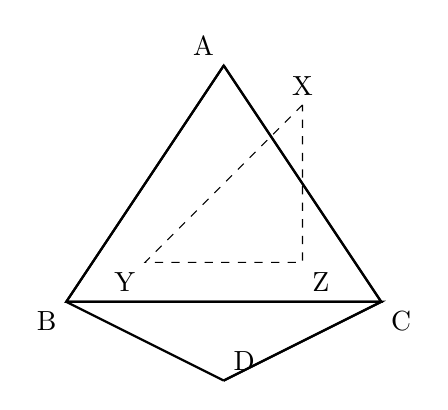
\begin{tikzpicture}[scale=2]
    % Draw the tetrahedron
    \coordinate (A) at (0, 1);
    \coordinate (B) at (-1, -0.5);
    \coordinate (C) at (1, -0.5);
    \coordinate (D) at (0, -1);

    \draw[thick] (A) -- (B) -- (C) -- cycle;
    \draw[thick] (A) -- (B) -- (D);
    \draw[thick] (A) -- (C) -- (D);
    \draw[thick] (B) -- (C) -- (D);

    % Label the vertices of the tetrahedron
    \node at (A) [above left] {A};
    \node at (B) [below left] {B};
    \node at (C) [below right] {C};
    \node at (D) [above right] {D};

    % Draw the dual triangle
    \coordinate (X) at (0.5, 0.75);
    \coordinate (Y) at (-0.5, -0.25);
    \coordinate (Z) at (0.5, -0.25);

    \draw[dashed] (X) -- (Y) -- (Z) -- cycle;

    % Label the vertices of the dual triangle
    \node at (X) [above] {X};
    \node at (Y) [below left] {Y};
    \node at (Z) [below right] {Z};
\end{tikzpicture}
\end{document}